\section{Instalacion y puesta en marcha}

En primer lugar, para instalar Django en una distribución ubuntu o debian necesitamos contar
con una instalación previa de Python. En este caso suponiendo que partimos de una instalacion
correcta de python 3.5 debemos instalar las siguientes librerias con pip.


\lstset{
  language=Bash,
}
\begin{lstlisting}
pip3 install django
pip3 install gunicorn
pip3 install psycopg2
\end{lstlisting}

Para crear un proyecto de django debemos ejecutar el siguiente comando dentro de la carpeta
donde queremos que se almacene

\begin{lstlisting}
django-admin startproject <nombre proyecto>
\end{lstlisting}

El cual nos genera la estructura basica del proyecto. Ahora entramos en esta carpeta y comprobamos 
que tenemos un directorio con el mismo nombre del proyecto y un archivo llamado manage.py. En este
directorio creamos una carpeta llamada templates, que sera la encargada de almacenar el código html
del proyecto.

\begin{lstlisting}
mkdir templates
\end{lstlisting}

Después entramos en el directorio que tiene el mismo nombre que el proyecto el archivo views.py

\begin{lstlisting}
cd <nombre proyecto
touch views.py
\end{lstlisting}

Al hacer esto nos tiene que quedar una estructura parecida a la siguiente

\begin{center}
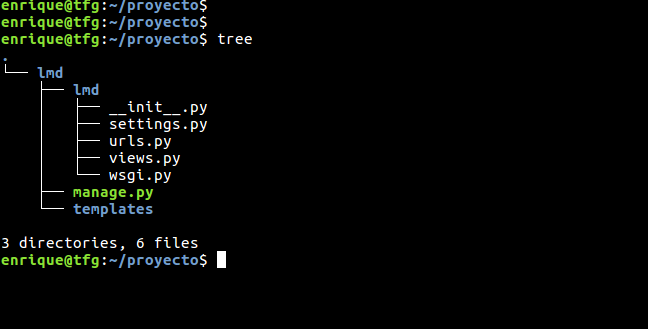
\includegraphics[scale=0.5]{img}
\captionof{figure}{Estructura proyecto}\label{fig:Estructura Proyecto}
\end{center}


